\scanpage{141}
p.ex. si l'image de $D'$ dans $Y$ est figurée par
\figure{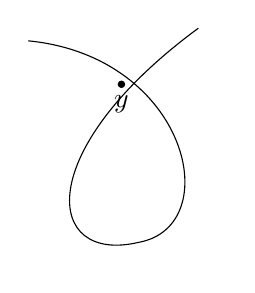
\begin{tikzpicture}[scale=.8]
\draw (-1.45,1.65) .. controls (1.1,1.4) and (1.7,-1.3) .. (.3,-1.55) .. controls (-1.2,-1.9) and (-1.4,-.1) .. (1.25,1.85);
\fill (.03,.96) circle (1.7pt);
\node[below] at (.03,.94) {$\unsure{y}$};
\end{tikzpicture}}, le voisinage tubulaire en question sera figuré \inserted{dans $Y$} par
\figure{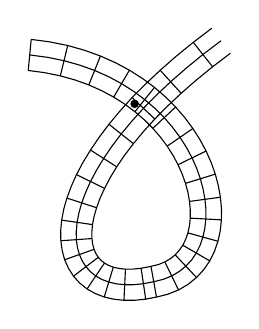
\begin{tikzpicture}[scale=.9,line width=.4pt]
\draw (-1.471,1.431) -- (-1.238,1.400) -- (-1.018,1.355) -- (-0.811,1.297) -- (-0.616,1.227) -- (-0.435,1.146) -- (-0.265,1.055) -- (-0.109,0.956) -- (0.035,0.849) -- (0.167,0.735) -- (0.287,0.615) -- (0.394,0.491) -- (0.490,0.363) -- (0.573,0.232) -- (0.643,0.101) -- (0.702,-0.031) -- (0.748,-0.162) -- (0.783,-0.291) -- (0.805,-0.417) -- (0.816,-0.538) -- (0.816,-0.653) -- (0.804,-0.761) -- (0.782,-0.861) -- (0.751,-0.952) -- (0.710,-1.035) -- (0.661,-1.107) -- (0.603,-1.171) -- (0.535,-1.225) -- (0.457,-1.271) -- (0.366,-1.308) -- (0.261,-1.333) -- (0.250,-1.336) -- (0.122,-1.360) -- (0.006,-1.372) -- (-0.099,-1.373) -- (-0.191,-1.363) -- (-0.271,-1.345) -- (-0.338,-1.319) -- (-0.395,-1.287) -- (-0.443,-1.249) -- (-0.482,-1.205) -- (-0.515,-1.154) -- (-0.542,-1.093) -- (-0.561,-1.022) -- (-0.572,-0.941) -- (-0.573,-0.848) -- (-0.564,-0.744) -- (-0.542,-0.630) -- (-0.506,-0.506) -- (-0.458,-0.373) -- (-0.394,-0.233) -- (-0.316,-0.084) -- (-0.222,0.071) -- (-0.113,0.232) -- (0.013,0.398) -- (0.156,0.570) -- (0.315,0.746) -- (0.492,0.925) -- (0.687,1.109) -- (0.899,1.294) -- (1.131,1.483) -- (1.380,1.673);
\draw (-1.450,1.650) -- (-1.202,1.617) -- (-0.966,1.569) -- (-0.744,1.506) -- (-0.534,1.431) -- (-0.338,1.344) -- (-0.154,1.245) -- (0.016,1.137) -- (0.173,1.020) -- (0.317,0.896) -- (0.448,0.765) -- (0.566,0.628) -- (0.671,0.488) -- (0.762,0.344) -- (0.841,0.197) -- (0.906,0.050) -- (0.958,-0.097) -- (0.997,-0.244) -- (1.023,-0.388) -- (1.036,-0.528) -- (1.035,-0.665) -- (1.021,-0.796) -- (0.994,-0.920) -- (0.954,-1.037) -- (0.900,-1.145) -- (0.834,-1.244) -- (0.753,-1.331) -- (0.660,-1.406) -- (0.553,-1.469) -- (0.433,-1.517) -- (0.300,-1.550) -- (0.300,-1.550) -- (0.154,-1.578) -- (0.018,-1.592) -- (-0.109,-1.593) -- (-0.227,-1.580) -- (-0.334,-1.555) -- (-0.432,-1.518) -- (-0.518,-1.469) -- (-0.593,-1.409) -- (-0.657,-1.338) -- (-0.709,-1.257) -- (-0.749,-1.166) -- (-0.777,-1.066) -- (-0.792,-0.957) -- (-0.793,-0.839) -- (-0.781,-0.712) -- (-0.756,-0.579) -- (-0.716,-0.438) -- (-0.661,-0.290) -- (-0.592,-0.136) -- (-0.507,0.024) -- (-0.407,0.189) -- (-0.291,0.360) -- (-0.159,0.535) -- (-0.010,0.714) -- (0.155,0.897) -- (0.338,1.083) -- (0.539,1.272) -- (0.758,1.463) -- (0.994,1.656) -- (1.250,1.850);
\draw (-1.429,1.869) -- (-1.165,1.834) -- (-0.914,1.783) -- (-0.677,1.716) -- (-0.452,1.635) -- (-0.241,1.541) -- (-0.043,1.435) -- (0.141,1.318) -- (0.311,1.192) -- (0.467,1.057) -- (0.609,0.915) -- (0.738,0.766) -- (0.852,0.612) -- (0.952,0.455) -- (1.039,0.294) -- (1.111,0.131) -- (1.169,-0.032) -- (1.212,-0.196) -- (1.241,-0.358) -- (1.256,-0.519) -- (1.255,-0.677) -- (1.239,-0.831) -- (1.206,-0.979) -- (1.157,-1.122) -- (1.091,-1.256) -- (1.006,-1.380) -- (0.904,-1.491) -- (0.785,-1.587) -- (0.650,-1.666) -- (0.501,-1.726) -- (0.339,-1.767) -- (0.350,-1.764) -- (0.187,-1.796) -- (0.030,-1.812) -- (-0.120,-1.812) -- (-0.263,-1.797) -- (-0.398,-1.766) -- (-0.525,-1.717) -- (-0.641,-1.652) -- (-0.744,-1.570) -- (-0.832,-1.472) -- (-0.903,-1.361) -- (-0.957,-1.240) -- (-0.992,-1.110) -- (-1.011,-0.972) -- (-1.013,-0.829) -- (-0.999,-0.681) -- (-0.970,-0.528) -- (-0.925,-0.370) -- (-0.865,-0.207) -- (-0.790,-0.039) -- (-0.699,0.133) -- (-0.592,0.308) -- (-0.470,0.488) -- (-0.332,0.672) -- (-0.177,0.858) -- (-0.005,1.048) -- (0.185,1.240) -- (0.391,1.434) -- (0.616,1.631) -- (0.858,1.828) -- (1.120,2.027);
\draw (-1.471,1.431) -- (-1.429,1.869);
\draw (-1.018,1.355) -- (-0.914,1.783);
\draw (-0.616,1.227) -- (-0.452,1.635);
\draw (-0.265,1.055) -- (-0.043,1.435);
\draw (0.035,0.849) -- (0.311,1.192);
\draw (0.287,0.615) -- (0.609,0.915);
\draw (0.490,0.363) -- (0.852,0.612);
\draw (0.643,0.101) -- (1.039,0.294);
\draw (0.748,-0.162) -- (1.169,-0.032);
\draw (0.805,-0.417) -- (1.241,-0.358);
\draw (0.816,-0.653) -- (1.255,-0.677);
\draw (0.782,-0.861) -- (1.206,-0.979);
\draw (0.710,-1.035) -- (1.091,-1.256);
\draw (0.603,-1.171) -- (0.904,-1.491);
\draw (0.457,-1.271) -- (0.650,-1.666);
\draw (0.261,-1.333) -- (0.339,-1.767);
\draw (0.122,-1.360) -- (0.187,-1.796);
\draw (-0.099,-1.373) -- (-0.120,-1.812);
\draw (-0.271,-1.345) -- (-0.398,-1.766);
\draw (-0.395,-1.287) -- (-0.641,-1.652);
\draw (-0.482,-1.205) -- (-0.832,-1.472);
\draw (-0.542,-1.093) -- (-0.957,-1.240);
\draw (-0.572,-0.941) -- (-1.011,-0.972);
\draw (-0.564,-0.744) -- (-0.999,-0.681);
\draw (-0.506,-0.506) -- (-0.925,-0.370);
\draw (-0.394,-0.233) -- (-0.790,-0.039);
\draw (-0.222,0.071) -- (-0.592,0.308);
\draw (0.013,0.398) -- (-0.332,0.672);
\draw (0.315,0.746) -- (-0.005,1.048);
\draw (0.687,1.109) -- (0.391,1.434);
\draw (1.131,1.483) -- (0.858,1.828);\fill (.03,.96) circle (1.7pt);\end{tikzpicture}}, et hors de $Y$ par
\figure{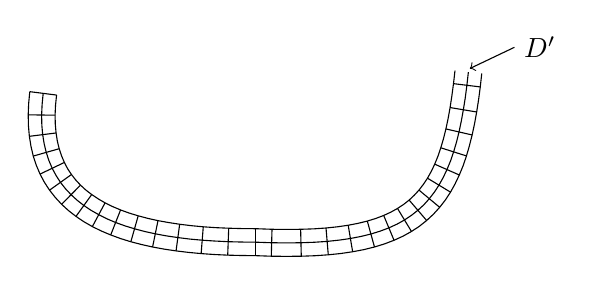
\begin{tikzpicture}[scale=.9,line width=.4pt]
\draw (-3.189,1.224) -- (-3.205,1.057) -- (-3.211,0.897) -- (-3.208,0.742) -- (-3.195,0.594) -- (-3.172,0.452) -- (-3.140,0.315) -- (-3.097,0.185) -- (-3.044,0.061) -- (-2.982,-0.056) -- (-2.910,-0.166) -- (-2.829,-0.269) -- (-2.740,-0.365) -- (-2.643,-0.454) -- (-2.537,-0.536) -- (-2.425,-0.612) -- (-2.306,-0.680) -- (-2.180,-0.742) -- (-2.047,-0.798) -- (-1.908,-0.849) -- (-1.763,-0.894) -- (-1.612,-0.933) -- (-1.456,-0.968) -- (-1.293,-0.998) -- (-1.125,-1.023) -- (-0.951,-1.044) -- (-0.771,-1.061) -- (-0.586,-1.074) -- (-0.396,-1.083) -- (-0.201,-1.088) -- (0.000,-1.090) -- (-0.008,-1.090) -- (0.219,-1.098) -- (0.436,-1.100) -- (0.642,-1.098) -- (0.838,-1.091) -- (1.023,-1.078) -- (1.199,-1.060) -- (1.367,-1.035) -- (1.525,-1.005) -- (1.675,-0.968) -- (1.817,-0.924) -- (1.951,-0.873) -- (2.078,-0.815) -- (2.197,-0.749) -- (2.308,-0.676) -- (2.411,-0.594) -- (2.507,-0.505) -- (2.595,-0.408) -- (2.675,-0.305) -- (2.748,-0.194) -- (2.813,-0.076) -- (2.872,0.048) -- (2.926,0.179) -- (2.973,0.317) -- (3.015,0.462) -- (3.053,0.613) -- (3.087,0.771) -- (3.117,0.937) -- (3.144,1.110) -- (3.168,1.291) -- (3.189,1.480);
\draw (-3.000,1.200) -- (-3.015,1.044) -- (-3.022,0.894) -- (-3.019,0.752) -- (-3.007,0.617) -- (-2.986,0.489) -- (-2.957,0.367) -- (-2.919,0.252) -- (-2.873,0.143) -- (-2.818,0.041) -- (-2.756,-0.056) -- (-2.685,-0.146) -- (-2.606,-0.230) -- (-2.520,-0.309) -- (-2.426,-0.382) -- (-2.325,-0.450) -- (-2.216,-0.512) -- (-2.101,-0.570) -- (-1.978,-0.622) -- (-1.848,-0.669) -- (-1.711,-0.711) -- (-1.568,-0.749) -- (-1.418,-0.782) -- (-1.262,-0.811) -- (-1.099,-0.835) -- (-0.931,-0.856) -- (-0.756,-0.872) -- (-0.575,-0.884) -- (-0.389,-0.893) -- (-0.197,-0.898) -- (0.000,-0.900) -- (0.000,-0.900) -- (0.224,-0.908) -- (0.436,-0.910) -- (0.637,-0.908) -- (0.828,-0.901) -- (1.007,-0.889) -- (1.176,-0.871) -- (1.335,-0.848) -- (1.484,-0.819) -- (1.624,-0.785) -- (1.756,-0.744) -- (1.878,-0.698) -- (1.992,-0.646) -- (2.098,-0.587) -- (2.196,-0.522) -- (2.287,-0.450) -- (2.372,-0.372) -- (2.449,-0.286) -- (2.520,-0.194) -- (2.585,-0.095) -- (2.644,0.011) -- (2.698,0.125) -- (2.748,0.246) -- (2.792,0.375) -- (2.832,0.511) -- (2.868,0.656) -- (2.900,0.808) -- (2.929,0.968) -- (2.956,1.137) -- (2.979,1.314) -- (3.000,1.500);
\draw (-2.811,1.176) -- (-2.826,1.030) -- (-2.832,0.892) -- (-2.829,0.763) -- (-2.818,0.641) -- (-2.800,0.526) -- (-2.774,0.419) -- (-2.741,0.319) -- (-2.701,0.225) -- (-2.655,0.137) -- (-2.601,0.055) -- (-2.540,-0.023) -- (-2.473,-0.095) -- (-2.398,-0.164) -- (-2.315,-0.228) -- (-2.225,-0.288) -- (-2.127,-0.345) -- (-2.021,-0.397) -- (-1.908,-0.445) -- (-1.787,-0.489) -- (-1.659,-0.528) -- (-1.523,-0.564) -- (-1.380,-0.596) -- (-1.230,-0.623) -- (-1.074,-0.647) -- (-0.910,-0.667) -- (-0.741,-0.683) -- (-0.564,-0.695) -- (-0.382,-0.703) -- (-0.194,-0.708) -- (0.000,-0.710) -- (0.008,-0.710) -- (0.229,-0.718) -- (0.437,-0.720) -- (0.633,-0.718) -- (0.818,-0.712) -- (0.991,-0.700) -- (1.153,-0.683) -- (1.304,-0.661) -- (1.444,-0.634) -- (1.574,-0.602) -- (1.694,-0.565) -- (1.805,-0.523) -- (1.906,-0.476) -- (2.000,-0.424) -- (2.085,-0.368) -- (2.164,-0.306) -- (2.236,-0.238) -- (2.303,-0.165) -- (2.365,-0.084) -- (2.423,0.003) -- (2.476,0.098) -- (2.525,0.201) -- (2.570,0.312) -- (2.611,0.432) -- (2.649,0.561) -- (2.683,0.698) -- (2.714,0.844) -- (2.742,1.000) -- (2.767,1.164) -- (2.790,1.337) -- (2.811,1.520);
\draw (-3.189,1.224) -- (-2.811,1.176);
\draw (-3.211,0.897) -- (-2.832,0.892);
\draw (-3.195,0.594) -- (-2.818,0.641);
\draw (-3.140,0.315) -- (-2.774,0.419);
\draw (-3.044,0.061) -- (-2.701,0.225);
\draw (-2.910,-0.166) -- (-2.601,0.055);
\draw (-2.740,-0.365) -- (-2.473,-0.095);
\draw (-2.537,-0.536) -- (-2.315,-0.228);
\draw (-2.306,-0.680) -- (-2.127,-0.345);
\draw (-2.047,-0.798) -- (-1.908,-0.445);
\draw (-1.763,-0.894) -- (-1.659,-0.528);
\draw (-1.456,-0.968) -- (-1.380,-0.596);
\draw (-1.125,-1.023) -- (-1.074,-0.647);
\draw (-0.771,-1.061) -- (-0.741,-0.683);
\draw (-0.396,-1.083) -- (-0.382,-0.703);
\draw (0.000,-1.090) -- (0.000,-0.710);
\draw (0.219,-1.098) -- (0.229,-0.718);
\draw (0.642,-1.098) -- (0.633,-0.718);
\draw (1.023,-1.078) -- (0.991,-0.700);
\draw (1.367,-1.035) -- (1.304,-0.661);
\draw (1.675,-0.968) -- (1.574,-0.602);
\draw (1.951,-0.873) -- (1.805,-0.523);
\draw (2.197,-0.749) -- (2.000,-0.424);
\draw (2.411,-0.594) -- (2.164,-0.306);
\draw (2.595,-0.408) -- (2.303,-0.165);
\draw (2.748,-0.194) -- (2.423,0.003);
\draw (2.872,0.048) -- (2.525,0.201);
\draw (2.973,0.317) -- (2.611,0.432);
\draw (3.053,0.613) -- (2.683,0.698);
\draw (3.117,0.937) -- (2.742,1.000);
\draw (3.168,1.291) -- (2.790,1.337);\draw[<-] (3.02,1.55)--(3.65,1.85) node[right] {$D'$};\end{tikzpicture}}.

Cette construction est possible dans le cadre (p.ex.) des \inserted{\unsure{paires (loc. fer.) de}} variétés différentiables, \inserted{paracompactes} en tant que germe de variété autour de $D'$ (défini à iso unique près ?...). Dans le cadre des \uline{multiplicités} \deleted{topologiques}, \inserted{\unsure{diff. (voire topologiques)},} on peut encore définir ce voisinage comme un germe de \deleted{topos}, \inserted{multiplicité diff.} par descente à partir d'une situation d'\deleted{espaces analytiques} \inserted{variétés diff. (ou top.)} paracompactes. On peut aussi, me semble-t-il, donner
\margin{140}
